% !TEX root = ../main.tex

\chapter{随机传值进程模型的应用}\label{ch:gossip}

如前文所述,传值进程模型可以用于对通信协议的形式刻画,
我们可以使用随机传值进程模型对引入了随机性的通信协议进行形式刻画。
本章中我们使用随机传值进程模型对基于云计算协议
Gossip-Style Membership协议的通信过程进行建模和模拟实现,
作为应用案例,以证明$\mathbb{RVPC}_{\mathsf{Th}}$对并发通信系统的建模和分析具有一定的可行性。

\section{Gossip-Style Membership协议}
\subsection{Gossip协议}
Gossip协议,也称为流言协议、传染病协议(Epidemic Protocol)是一个基于传染病传播方式的点对点通信协议\cite{Gossip}。

Gossip协议可以被解释为办公室流言的传播:
每一个职员会随机和另一个职员分享最近的流言,
被分享者得知流言后会随机的和其他人分享,
在一次分享中,被分享者或许已经知道了这个流言。
比如有一天,小赵传出老板的一个谣言,
他在一次会议结束时将这个谣言告诉了小钱;
小钱得知了谣言后,又在一次会议后将它告诉了小李;
小李在一次会议后告诉小孙时,
发现小孙已经从小王那里知道了这个谣言。

Gossip协议
主要作分布式数据库系统中各个副本节点同步数据之用,
这种场景的一个最大特点就是组成的网络的节点都是对等节点,
是非结构化网络。
2015年之前,Bitcoin就是使用了Gossip协议来传播交易信息\cite{Bitcoin}。

Gossip协议中,节点之间的通信方式有三种:
\begin{itemize}
   \item[(1)] {
      {\bfseries Push Gossip:} 
      
      消息的发送者周期性的随机选择$k$个目标节点发送Gossip Message。
      接收到Gossip Message的节点可以根据本地时间,
      周期性的选择$k$个目标节点发送Gossip Message。
      在发送过程中,
      已经拥有Gossip Message的节点仍然可以被选为目标节点。
   }
   \item[(2)] {
      {\bfseries Pull Gossip:}

      每个节点周期性的向$k$个目标节点发送Gossip Query,
      收到Gossip Query的节点若拥有Gossip Message的节点会向发送Query的节点返回Gossip Message的拷贝。
   }
   \item[(3)] {
      {\bfseries Push/Pull Gossip:}

      在超过$\frac{n}{2}$的节点拥有Gossip Message时,可以证明此时选择Pull Gossip会比Push Gossip传播的更快\cite{Gossip}。
      因此在使用Gossip协议时,常使用Push Gossip与Pull Gossip的混合:
      在消息传播$\frac{n}{2}$节点之前使用Push Gossip,在消息传播$\frac{n}{2}$之后使用Pull Gossip。
   }
\end{itemize}

\subsection{组成员协议}

组成员协议(Group Membership Protocol,后文简称Membership协议)\cite{Membership}为集群中的每个节点提供了一个本地的列表,
称为Membership List,用来维护集群中其他节点的信息。
Membership协议提供了两个主要的服务:
\begin{itemize}
   \item[(1)] 检测失效的节点
   \item[(2)] 传播消息,如:告知其他节点失效信息
\end{itemize}

常见的Membership协议有
Heartbeating Protocol\cite{Heartbeat}, 
Gossip-Style Membership Protocol\cite{Gossip_style}, 
SWIM Failure Detector Protocol\cite{SWIM}等。

\section{基于Gossip-Style Membership协议的通信系统的实现}
我们使用$\mathbb{RVPC}_{\mathsf{Th}}$来实现Gossip-Style Membership协议\cite{Gossip_style},
来作为使用随机传值进程模型建模通信过程的示例,
类似的,也可以使用同样的建模方法建模其他现实问题。

由于Membership可以看作节点内部的功能,我们可以首先实现Gossip协议,将网络建立起来。

\subsection{基于Gossip协议的通信系统的实现}\label{ch:gossip_impl}
由于Push Gossip的机制比较简单,
并且单一的Push Gossip协议仍然可以达到$O(\log N)$时间复杂度的消息传播\cite{Gossip},
本节我们使用$\mathbb{RVPC}_{\mathsf{Th}}$来建模以Push Gossip作为通信机制的Gossip协议。

我们首先来建模以Gossip协议为通信的Peer-to-Peer Sysyem的节点。
根据根据Gossip协议的定义,
我们可以从单一节点周期性的发送消息,
这意味着我们需要一个计时器机制,
我们选择在节点外部使用计时器周期性的通知节点发送消息,
节点的$\overline{time}$端口用于向计时器设置计时开始,
$timeout$端口用于接收计时器传来的timeout信号。
由于节点本身不产生和存储消息,
我们需要使用$accept$端口接收P2P系统外界消息,
使用$\overline{deliver}$向P2P系统外界传递节点在P2P系统中从其他节点收到的消息。
由于现实网络是复杂的,
我们将每一对节点之间的消息传播路径抽象为单独的、单工的通道,
如节点$Node_i$向$Node_j$传播消息时,
消息会在$trans_{i,j}$通道中,
从$Node_i$节点的$\overline{trans_{i,j}}$端口发出,
从$Node_j$节点的$trans_{i,j}$端口接收。
这里的消息传输方式实际上是信息的逻辑传输路径,
信息的物理传输路径可能是十分复杂且动态的,
我们可以将系统中节点的编号简单的理解为Socket通信中的IP地址:端口号,
每一个节点代表了某台主机上的某个进程。

Gossip单节点的通道示意图如图~\ref{fig:gossip_node_1}和
以Gossip协议作为通信协议的四节点的Peer-to-Peer Sysyem的示意图如图
~\ref{fig:p2p_system}。

\begin{figure}[!htp]
   \begin{minipage}{0.3\textwidth}
   \centering
   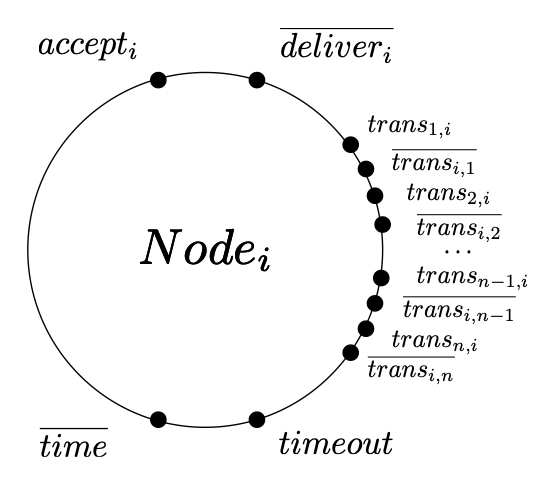
\includegraphics[width=5cm]{../figures/Node_gossip2.png}
   \caption{Gossip 节点示意图}
  \label{fig:gossip_node_1}
\end{minipage}\hfill
\begin{minipage}{0.6\textwidth}
   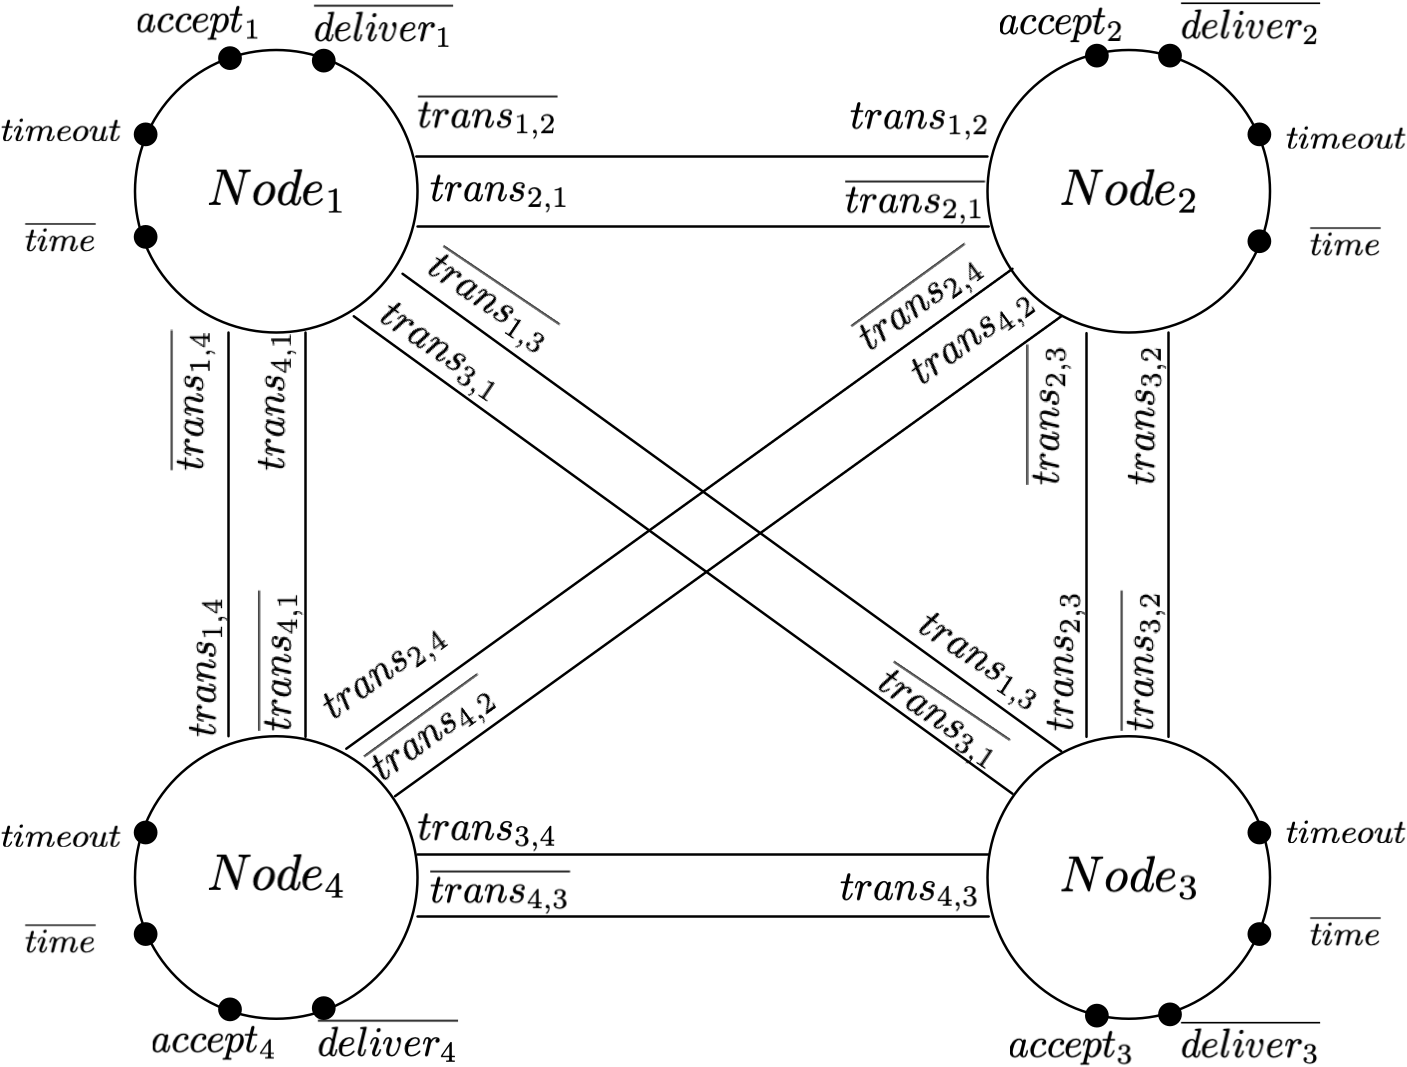
\includegraphics[width=8cm]{../figures/GossipSystem.png}
   \caption{基于Gossip协议的四节点P2P系统结构}
   \label{fig:p2p_system}
\end{minipage}
 \end{figure}

Gossip节点Node的状态有以下几种,分别对应Gossip协议中节点的状态:
\begin{table}[!hpt]
    \caption{节点状态对应表}
    \label{tab:firstone}
    \centering
    \begin{tabular}{@{}llr@{}} \toprule
    %   \multicolumn{2}{c}{Item} \\ \cmidrule(r){1-2}
      节点状态 & Gossip状态 \\ \midrule
      Node&可接受系统外信息(除此状态其余状态均无法接收外界信息)\\
      DeliveringNode&可向系统外传递信息\\
      UnInfectiousNode&未获取Gossip Message\\
      InfectiousNode&已获取Gossip Message\\
      GossipingNode&可向系统内部特定b个其他节点发送Gossip Message\\ \bottomrule
    \end{tabular}
  \end{table}

基于以上定义的节点结构和节点状态,
我们定义一个基于Gossip协议的P2P系统。
\begin{equation}
   \begin{split}
   Node_i& \stackrel{def}{=} accept_i(x).DeliveringNode_i(x)\\
   DeliveringNode_i(x) &\stackrel{def}{=} \overline{deliver_i}(x).InfectiousNode_i(x)\\
   InfectiousNode_i(x)&\stackrel{def}{=}timeout.(\bigoplus_{perm\in \mathsf{PERM}_i} p_{perm}\tau.GossipingNode_{i,perm}(x))\\
%    &+\sum_{j\in \mathsf{N}/\{i\}}trans_{j,i}(x).DeliveringNode_i(x)\\
   GossipingNode_{i,perm}(x)&\stackrel{def}{=}\overline{trans_{i,perm_{1}}}(x).\dots \overline{trans_{i,perm_{b}}}(x).\overline{time}.InfectiousNode_i(x)\\
   UnInfectiousNode_i &\stackrel{def}{=} \sum_{j\in \mathsf{N}/\{i\}}trans_{j,i}(x).DeliveringNode_i(x)\\
   GossipSystem_\mathsf{N}&\stackrel{def}{=}(Node_1\mid UnInfectiousNode_2\mid \dots \mid UnInfectiousNode_n)\\
   &\backslash \{trans_{i,j}\mid i\in \mathsf{N} \wedge j\in \mathsf{N} \wedge i\neq j\}\cup \{time, timeout\}
   \end{split}
\end{equation}
在这个P2P系统中共有$n$个节点,标号为$\mathsf{N}=\{1,2,\dots, n\}$,
每一个拥有Gossip Message的节点周期性的向$\mathsf{k}(\mathsf{k}\leq n-1)$
个其他节点发送Gossip Message。
其中$\mathsf{PERM}_i$为$\mathsf{N}/\{i\}$中任选$\mathsf{k}$个元素的全排列,
$p_{\mathsf{perm}}$为向一个特定的排列$perm$发送Gossip Message的概率,
为了方便建模,
我们假设一个节点选择任意其他节点作为Gossip的目标节点的概率是相同的,
即$p_{perm} = \frac{1}{A_{n-1}^{\mathsf{k}}} = \frac{(n-\mathsf{k}-1)!}{(n-1)!}$为固定值,
当$\mathsf{k}=2$时,$p_{perm} = \frac{1}{(n-1)(n-2)}$。

我们可以看到节点$Node_i$接受到外界消息$x$后,
迁移为$DeliveringNode_i(x)$的状态,
向外界递送这个消息,
进而迁移为$InfectiousNode)i(x)$的状态,
可以在接受到$timeout$信号时以概率$p_{\mathsf{perm}}$
的概率选定$\mathsf{N}/\{i\}$中任选$\mathsf{k}$个元素的全排列
中的一个排列$perm$作为发送目标,
进而迁移为$GossipingNode_{i,perm}(x)$,
向$perm$中的节点发送Gossip Message,
发送完成后回到$InfectiousNode_i(x)$的状态。
在一个$GossipSystem_{\mathsf{N}}$中,
还有状态为$InfectiousNode_i$的节点,
这些节点在接受了来自其他节点的Gossip Message时会迁移到$DeliveringNode_i(x)$的状态。
为了后面的分析,上述定义基于一系列理想条件的假设:
\begin{itemize}
   \item [(1)] {网络传输可靠。
   然而现实中的网络传输存在丢包、延迟、比特反转等问题,
   我们可以通过ACK机制来解决。
   对不可靠网络下的Gossip协议,我们可以在上述理想条件下增加对网络传输的过程的建模,建模过程在MILNER R的CCS中有提及
   \cite{Milner_CCS}。
   }
   \item [(2)] {节点不会损坏。
   在现实中节点(主机)在运行了一定时间后就会出现问题,
   对于多个节点构成的P2P系统,
   存在节点失效的概率只会更高\cite{MTTF},
   Membership协议就是用来探测节点失效的一种方式。
   }
   \item [(3)] {
      系统中只存在一个消息的传输。
      对于单个消息源的多个消息,我们仍然可以看作单个Gossip Message一起发送;
      对于多个消息源,我们可以为每个节点提供消息队列机制来保存多个消息,
      后文对Membership的建模提供了一个多消息源的解决思路。
      }
\end{itemize}

\subsection{Gossip协议的等价性}
% Brewer在CAP定理[cite]说到,
% 在分布式环境中设计和部署应用程序时,
% 存在特殊关系中的三个核心系统需求,
% 分别是一致性、可用性和分区容忍度。
% 其中一致性指一致性是指分布式系统中的多个服务节点,给定一系列的操作,在约定协议的保障下,使它们对外界呈现的状态是一致的。
% 分布式系统中的一致性按照对一致性要求的不同,主要分为严格一致性,强一致性,弱一致性和最终一致性这四大类。
% Gossip协议具有最终一致性。

Gossip协议的目的是为了在系统内对节点进行多播,
我们可以定义一个多播的规约,
证明~\ref{ch:gossip_impl}节中我们使用$\mathbb{RVPC}_{\mathsf{Th}}$实现的基于Gossip协议的P2P系统满足这个规约,
在进程演算中,我们需要证明二者互模拟。
由于我们在~\ref{ch:gossip_impl}节中实现的是单消息源单个消息的传播,
在多播的定义中同样我们只关注单消息源单个消息的多播。
\begin{definition} 单消息源的多播规约定义如下:
\begin{equation} 
   \begin{split}
    MulticastSpec_\mathsf{N}&\stackrel{def}{=}accept_1(x).\overline{deliver_1}(x).Multicasting_{\mathsf{N},\{1\}}(x)\\
    Multicasting_{\mathsf{N},\mathsf{KNOWN}}(x)&\stackrel{def}{=}\overline{deliver_i}(x).Multicasting_{\mathsf{N},\mathsf{KNOWN}\cup\{i\}}(x), \\
    &i\in \mathsf{N}-\mathsf{KNOWN} \wedge |\mathsf{N}|\neq |\mathsf{KNOWN}|
   \end{split}
   \end{equation}
\end{definition} 
其中$|\mathsf{KNOWN}|$为已经得到此消息的节点编号集合,
节点可以通过$deliver$通道告知通信系统外(如本地的其他进程)节点已收到信息。
若一个节点对系统外通过$deliver$通道传递了这个消息,
我们将这个节点加入$|\mathsf{KNOWN}|$,
表示这个节点已经收到了消息。

 \begin{definition} 
   由于$GossipSystem_{\mathsf{N}}$中的节点可能处于:$InfectiousNode$,$DeliveringNode$,$UnInfectiousNode$
   三种状态(我们将$GossipingNode$的状态合并进了$InfectiousNode$),
   在后续的证明过程中表示起来比较冗长,
   为了方便后续的证明,我们给出特定状态下的
   $GossipSystem_{\mathsf{N}}$的记法,
   其中Composition算子符合交换律。
    \begin{equation}
      \begin{split}
   &GossipSystem_{\mathsf{N},(a,b,c)}(x)\\
   &= (\stackrel{a}{\overbrace{InfectiousNode(x)\mid \dots \mid InfectiousNode(x)}}\\
   &\mid \stackrel{b}{\overbrace{DeliveringNode(x)\mid \dots\mid DeliveringNode(x)}}\\
   &\mid \stackrel{c}{\overbrace{UnInfectiousNode\mid \dots \mid UnInfectiousNode}})\\
   &\backslash \{trans_{i,j}\mid i\in \mathsf{N} \wedge j\in \mathsf{N} \wedge i\neq j\}\cup \{time, timeout\}
      \end{split}
\end{equation}
 \end{definition}
 其中,$GossipSystem_{\mathsf{N},(a,b,c)}(x)$表示
 在系统的$n=|\mathsf{N}|$个节点中,有$a$个处于$InfectiousNode(x)$的状态,
 有$b$个处于$DeliveringNode(x)$的状态,
 有$c$个处于$UnInfectiousNode$的状态,
 且满足$a+b+c=n$。
 很显然,初始的$GossipSystem_{\mathsf{N}}$中唯一的$Node$状态的节点此时已经从外界接收了某个消息$x$。

 接下来我们来证明,我们实现的基于Gossip协议的P2P系统满足多播系统的规约。
 由于$GossipSystem_{\mathsf{N}}$和$MulticastSpec_\mathsf{N}$中的每一个节点能且仅能执行一次$deliver$操作,
 且$deliver$的顺序不影响功能,
所以我们可以规定$A\stackrel{\overline{deliver_i}(t_1)}{\longrightarrow}_{\top} B$和$C\stackrel{\overline{deliver_j}(t_2)}{\longrightarrow}_{\top}B$是互模拟的当且仅当$t_1=t_2$,对下标是否一致不作要求。
因此在后文的证明中忽略了下标。
\begin{theorem}
    $GossipSystem_{\mathsf{N}} =_{\mathbb{RVPC}_{\mathsf{Th}}} MulticastSpec_{\mathsf{N}}$,$\mathsf{Th}$是可判定的逻辑。
\end{theorem}
\begin{proof}

我们可以通过构建等价集,并证明等价集是一个符号互模拟关系
来证明$GossipSystem_{\mathsf{N}} =_{\mathbb{RVPC}_{\mathsf{Th}}} MulticastSpec_{\mathsf{N}}$。

构造等价集
\begin{equation}
   \begin{split}
      \mathcal{S}&=\{(GossipSystem_{\mathsf{N}}, MulticastSpec_{\mathsf{N}}), \\
      &(GossipSystem_{\mathsf{N},(n,0,0)}(x), Multicasting_{\mathsf{N},\mathsf{N}}(x))\}\\
      & \cup \{(GossipSystem_{\mathsf{N},(a,b,c)}(x), Multicasting_{\mathsf{N}, \mathsf{KNOWN}}(x))\mid |\mathsf{KNOWN}| = a\neq n\}
   \end{split}
\end{equation}

我们来依次证明$\mathcal{S}$中的每一对等价关系为符号互模拟关系:
\begin{itemize}
    \item[(1)] {
       $GossipSystem_{\mathsf{N},(n,0,0)}(x)$和$Multicasting_{\mathsf{N},\mathsf{N}}(x)$的$\top \mathcal{S}$条件等价树分别只有一个根节点,
       且不能转移至其他等价集,他们的互模拟是显然的,实际上$GossipSystem_{\mathsf{N},(n,0,0)}(x)=Multicasting_{\mathsf{N},\mathsf{N}}(x)=0$。
    }
    \item[(2)] {
        对于$(GossipSystem_{\mathsf{N},(a,b,c)}(x), Multicasting_{\mathsf{N}, \mathsf{KNOWN}}(x))\mid |\mathsf{KNOWN}| = a\neq n$:

        % 对应的$Multicasting_{\mathsf{N}, \mathsf{KNOWN}}(x)\rightsquigarrow_{\top\mathcal{S}}\stackrel{\overline{deliver}(x)}{\longrightarrow}_{\top\mathcal{S}} []$
        \begin{itemize}
            \item[(a)] {若$a<n-1$:
            $GossipSystem_{\mathsf{N},(a,b,c)}(x)$的$\top \mathcal{S}$条件等价树 $t$如图~\ref{fig:epsilon_1}所示。
            \begin{figure}[!htbp]
            	\small
            	\centering
            	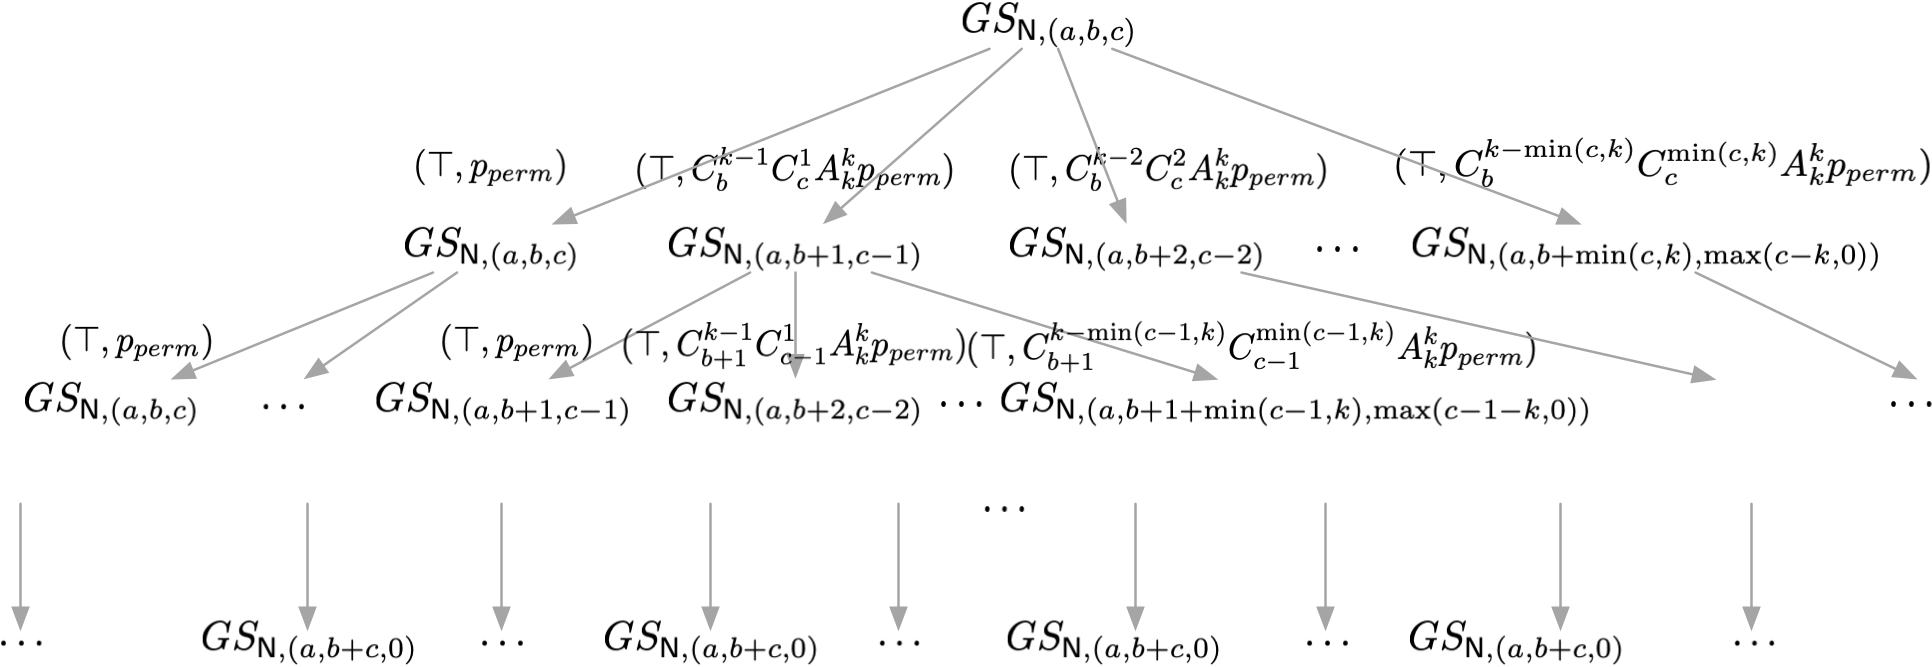
\includegraphics[width=14cm]{../figures/epsilon_tree1.png}
                \caption{$GossipSystem_{\mathsf{N},(a,b,c)}(x)$关于$\top\mathcal{S}$的条件等价树 $t$}
                \label{fig:epsilon_1}
            \end{figure}
            当$t$上的节点进入$GossipSystem_{\mathsf{N},(a,b+c,0)}(x)$状态时,
            状态保持的静态迁移($\tau$动作)就会终止,
            因此$GossipSystem_{\mathsf{N},(a,b+c,0)}(x)$为$t$的叶子结点。
            很显然,对$t$上的每一个非叶结点,都会经过$Node_j\stackrel{p'_j}{\rightarrow}_{\top}GossipSystem_{\mathsf{N},(a,b+c,0)}(x),p'_j=p_{j_1}p_{j_2}\dots p_{j_m}<1$。
            对$t$的叶子结点有$GossipSystem_{\mathsf{N},(a,b+c,0)}(x)\stackrel{\overline{deliver}(x)}{\longrightarrow}_{\top} GossipSystem_{\mathsf{N},(a+1,b+c-1,0)}(x)$。
            即
            $$GossipSystem_{\mathsf{N},(a,b,c)}(x)\rightsquigarrow_{\top\mathcal{S}}\stackrel{\overline{deliver}(x)}{\longrightarrow}_{\top}[GossipSystem_{\mathsf{N},(a+1,b',c')}(x)]_{\top\mathcal{S}}$$
            其中$b'+c'=b+c-1$。
            我们可以用$$Multicasting_{\mathsf{N},\mathsf{KNOWN}}\rightsquigarrow_{\top\mathcal{S}}\stackrel{\overline{deliver}(x)}{\longrightarrow}_{\top} Multicasting_{\mathsf{N}, \mathsf{KNOWN}'}$$来模拟上述状态迁移。
            对称的模拟依然成立。
            }
            \item[(b)] {若$a=n-1$:
             
                  若$b=1$,
                  $GossipSystem_{\mathsf{N},(n-1,1,0)}(x)$的$\top \mathcal{S}$条件等价树 $t$只有一个根节点,对于
                  $(GossipSystem_{\mathsf{N},(n-1,1,0)}(x)\rightsquigarrow_{\top\mathcal{S}}\stackrel{\overline{deliver}(x)}{\longrightarrow}_{\top}[GossipSystem_{\mathsf{N},(n,0,0)}(x)]_{\top\mathcal{S}}$,
                  我们可以用$Multicasting_{\mathsf{N},\mathsf{KNOWN}}\rightsquigarrow_{\top\mathcal{S}}\stackrel{\overline{deliver}(x)}{\longrightarrow}_{\top} Multicasting_{\mathsf{N}, \mathsf{N}}$来模拟。
               
                  若$b=0$,  
                  $GossipSystem_{\mathsf{N},(n-1,0,1)}(x)$的$\top \mathcal{S}$条件等价树 $t$如图~\ref{fig:epsilon_2}所示。
                  \begin{figure}[!htbp]
                     \small
                     \centering
                     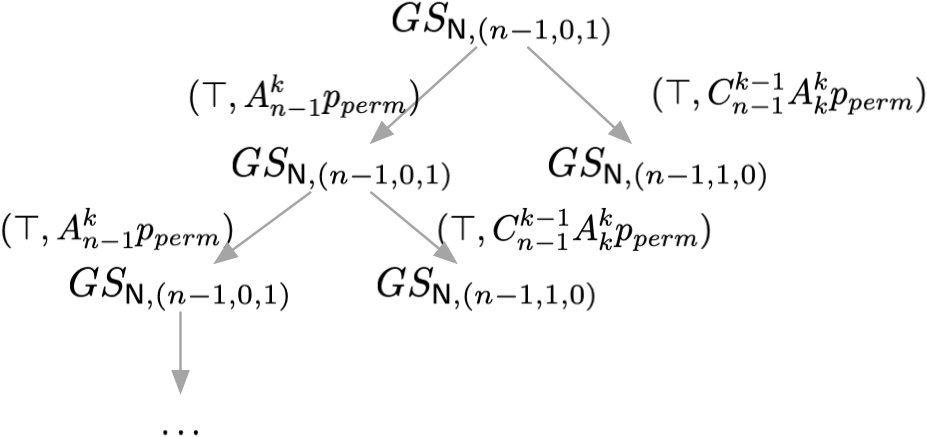
\includegraphics[width=8cm]{../figures/epsilon_tree_2.png}
                      \caption{$GossipSystem_{\mathsf{N},(a,b,c)}(x)$关于$\top\mathcal{S}$的条件等价树 $t$}
                      \label{fig:epsilon_2}
                  \end{figure}
                  
                  $GossipSystem_{\mathsf{N},(n-1,1,0)}$为$t$的叶节点,
                  且有$(GossipSystem_{\mathsf{N},(n-1,0,1)}(x)\rightsquigarrow_{\top\mathcal{S}}\stackrel{\overline{deliver}(x)}{\longrightarrow}_{\top}[GossipSystem_{\mathsf{N},(n,0,0)}(x)]_{\top\mathcal{S}}$。
                  我们可以用$Multicasting_{\mathsf{N},\mathsf{KNOWN}}\rightsquigarrow_{\top\mathcal{S}}\stackrel{\overline{deliver}(x)}{\longrightarrow}_{\top} Multicasting_{\mathsf{N}, \mathsf{N}}$来模拟。
            }
        \end{itemize}
    }
    \item[(3)] {
        对$(GossipSystem_{\mathsf{N}}, MulticastSpec_{\mathsf{N}})$,
        我们可以用$$GossipSystem_{\mathsf{N}}\stackrel{accept(x).\overline{deliver(x)}}{\longrightarrow}_{\top}GossipSystem_{\mathsf{N},(1,0,0)}(x)$$
        $$MulticastSpec_{\mathsf{N}}\stackrel{accept(x).\overline{deliver(x)}}{\longrightarrow}_{\top}Multicasting_{\mathsf{N},\{1\}}$$来相互模拟。
    }
 \end{itemize}
\end{proof}
\subsection{基于Gossip-Style Membership协议的通信系统的实现}\label{ch:membership_system}

Van RENESSE R提出了一种基于Gossip协议的错误检测机制:
在集群中的每一个节点会维护一个列表Membership List,列表中包含已知的其他节点的\textit{地址}和整数表示的\textit{心跳}。
在每一个Gossip的周期,节点会增加自己的心跳,
并且随机的向另一个节点发送自己的Membership List;
若节点收到了其他节点发送过来的Membership List,
它会将两个列表合并,保留对应地址心跳最大的项。
若节点的Membership List的一项经过$T_{fail}$时间没有更新,则认为这一项对应的节点失效\cite{Gossip_style},
我们称为Gossip-Style Membership 协议。

在本次的实现中,我们规定在每一个Gossip周期中,
节点可以随机选择$k$个节点发送自己的Membership List。

由于Gossip-Style Membership无需与外界的输入输出,并且需要提供储存、更新Membership List的函数,
我们需要对之前的节点结构进行调整。
同时,系统内的节点也会有失效的可能,我们可以用$p_{fail}$来定义一个节点失效的概率,
同时经过一个静态迁移$\tau$,这个节点就会被修复。
另外,由于在系统中的所有节点都是消息源,
且Membership List在系统中不停的更新,
因此也没有了感染者与被感染者的角色区分,
也需要对名称进行了修改。
\begin{figure}[!htbp]
	\small
	\centering
	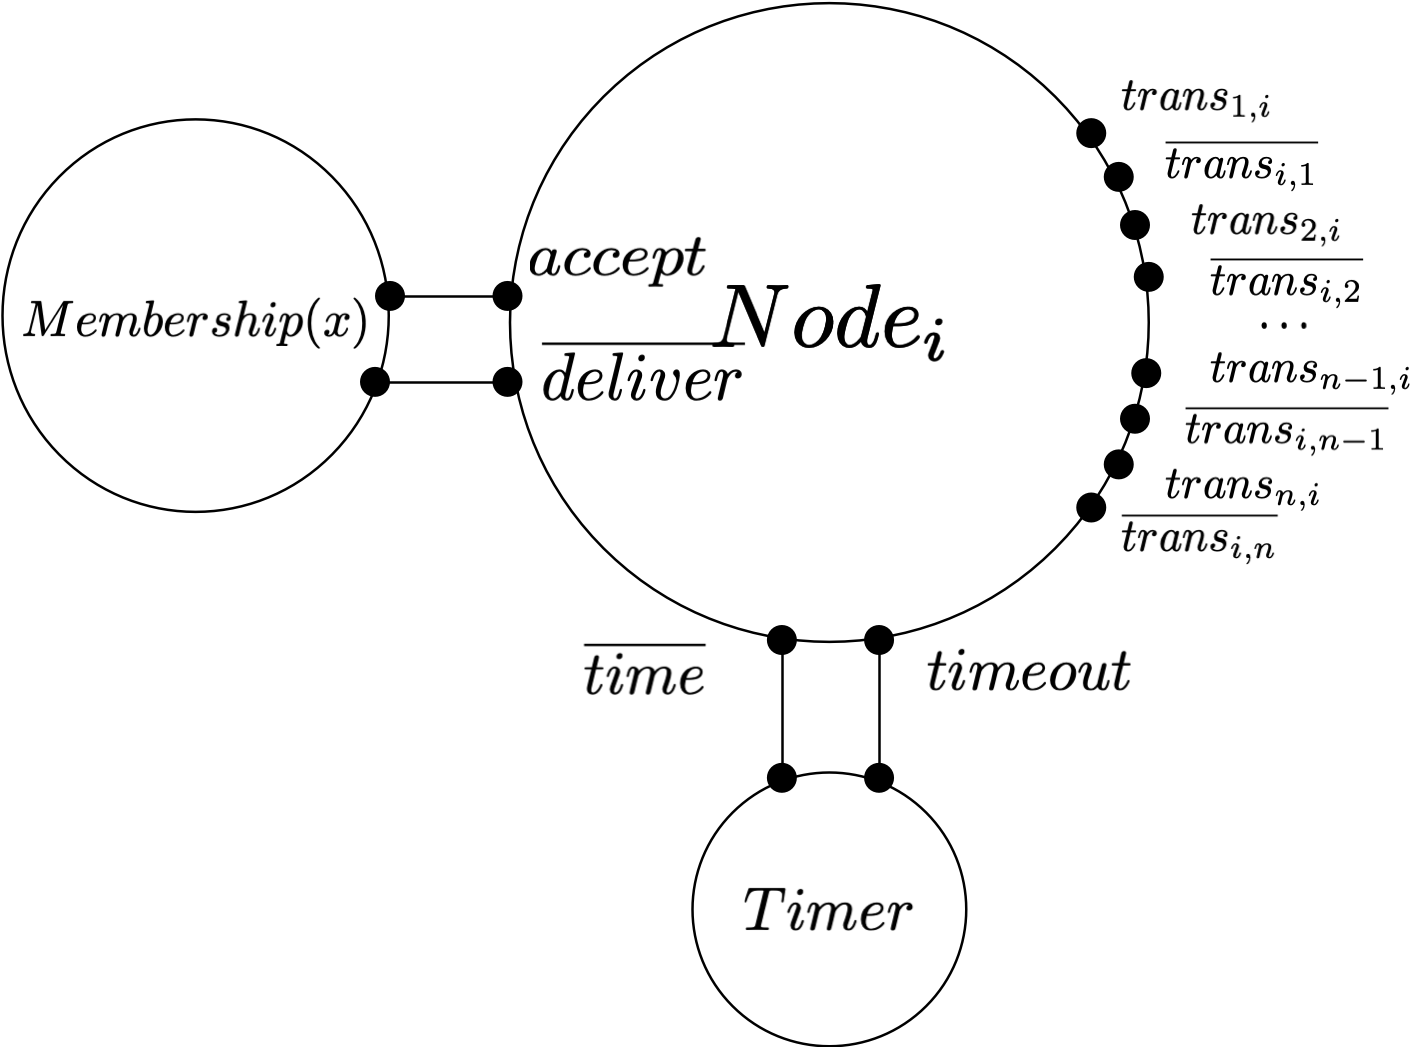
\includegraphics[width=6cm]{../figures/Node.png}
    \caption{Gossip-Style Membership节点示意图}
    \label{fig:membership_node}
\end{figure}
在Gossip System节点的基础上,
将原本对外暴露的$accept,deliver$通道用于连接$Membership$,
作为链接网络的节点获取和更新本地Membership List的通道,
修改后的节点如图
\ref{fig:membership_node}
所示。

Gossip-Style Membership协议中的P2P系统定义如下,
\begin{equation}\label{eq:network_system}
   \begin{split}
    FragileNode_i&\stackrel{def}{=}p_{fail}\tau.BadNode_i\oplus (1-p_{fail})\tau.Node_i\\
    BadNode_i&\stackrel{def}{=}\tau.FragileNode_i\\
    Node_i&\stackrel{def}{=}timeout.accept(x).(\bigoplus_{perm\in \mathsf{PERM}_i} p_{perm}\tau.GossipingNode_{i,perm}(x))\\
     &+\sum_{j\in \mathsf{N}/\{i\}}trans_{j,i}(x).\overline{deliver}(x).FragileNode_i\\
    GossipingNode_{i,perm}(x)&\stackrel{def}{=}\overline{trans_{i,perm_{1}}}(x).\dots \overline{trans_{i,perm_{b}}}(x).\overline{time}.FragileNode_i\\
    GossipSystem_\mathsf{N}&\stackrel{def}{=}(FragileNode_1\mid FragileNode_2\mid \dots \mid FragileNode_n)\\
    &\backslash \{trans_{i,j}\mid i\in \mathsf{N} \wedge j\in \mathsf{N} \wedge i\neq j\}\cup \{time, timeout, accept, deliver\}
   \end{split}
   \end{equation}
 其中,每一个节点定义为$FragileNode$,每一时刻
 它会有$p_{fail}$的概率成为失效节点$BadNode$,
 和$1-p_{fail}$的概率成为可发送列表和接受列表的正常节点$Node$。
 在$Node$状态的节点,
 可以在外界计时器发送$timeout$信号时通过$accept$通道获取自身的
 Membership List,
 以概率$p_{\mathsf{perm}}$
 的概率选定$\mathsf{N}/\{i\}$中任选$\mathsf{k}$个元素的全排列
 中的一个排列$perm$作为发送目标,
 进而迁移为$GossipingNode_{i,perm}(x)$,
 向$perm$中的节点发送Membership List,
 发送完成后回到$FragileNode$的状态。
 一个有$n=|\mathsf{N}|$个节点的
 基于Gossip-Style Membership协议的P2P系统定义为
 $GossipSystem_{\mathsf{N}}$,
 它由$n$个$FragileNode$状态的并发的节点构成。

 此外,我们还需要定义每个节点本地的Membership系统,
 来处理Membership List的获取和更新。
 Membership List的内容一般为表~\ref{tab:membership_list}中的内容。
\begin{table}[!hpt]
    \caption{Membership List样表}
    \label{tab:membership_list}
    \centering
    \begin{tabular}{@{}ccc@{}} \toprule
    %   \multicolumn{2}{c}{Item} \\ \cmidrule(r){1-2}
      Address & HeartBeat & LocalTime \\ \midrule
      1 & 10120 & 66\\
      2 & 10103 & 62\\
      3 & 10098 & 63\\ \bottomrule
    \end{tabular}
  \end{table}
其中Address表示系统中其他节点的地址,HeartBeat表示对应节点的心跳计数,
LocalTime表示Membership List中这一项记录最近一次的更新时间,
当当前时间与某一项的LocalTime相差超过$T_{fail}$,
我们认为这一节点失效。

因此Membership系统需要有一个本地计时器Timer、一个心跳计数器Counter,
一个本地$MembershipList(X)$,
$X$应为一个(Address, HeartBeat, LocalTime)
的三元组的数组,
一个记录本地地址的$AddrInfo(address)$
(地址应在加入网络时由DNS分配,此处不考虑它的分配过程)。
定义$x_i[Address]$为取Address的值的操作子,
$x_i[HeartBeat]$同理。
$n$为MembershipList的最大容量。

我们定义的Membership系统的实现如图~\ref{fig:membership_system}所示,
\begin{figure}[!htbp]
	\small
   \centering
	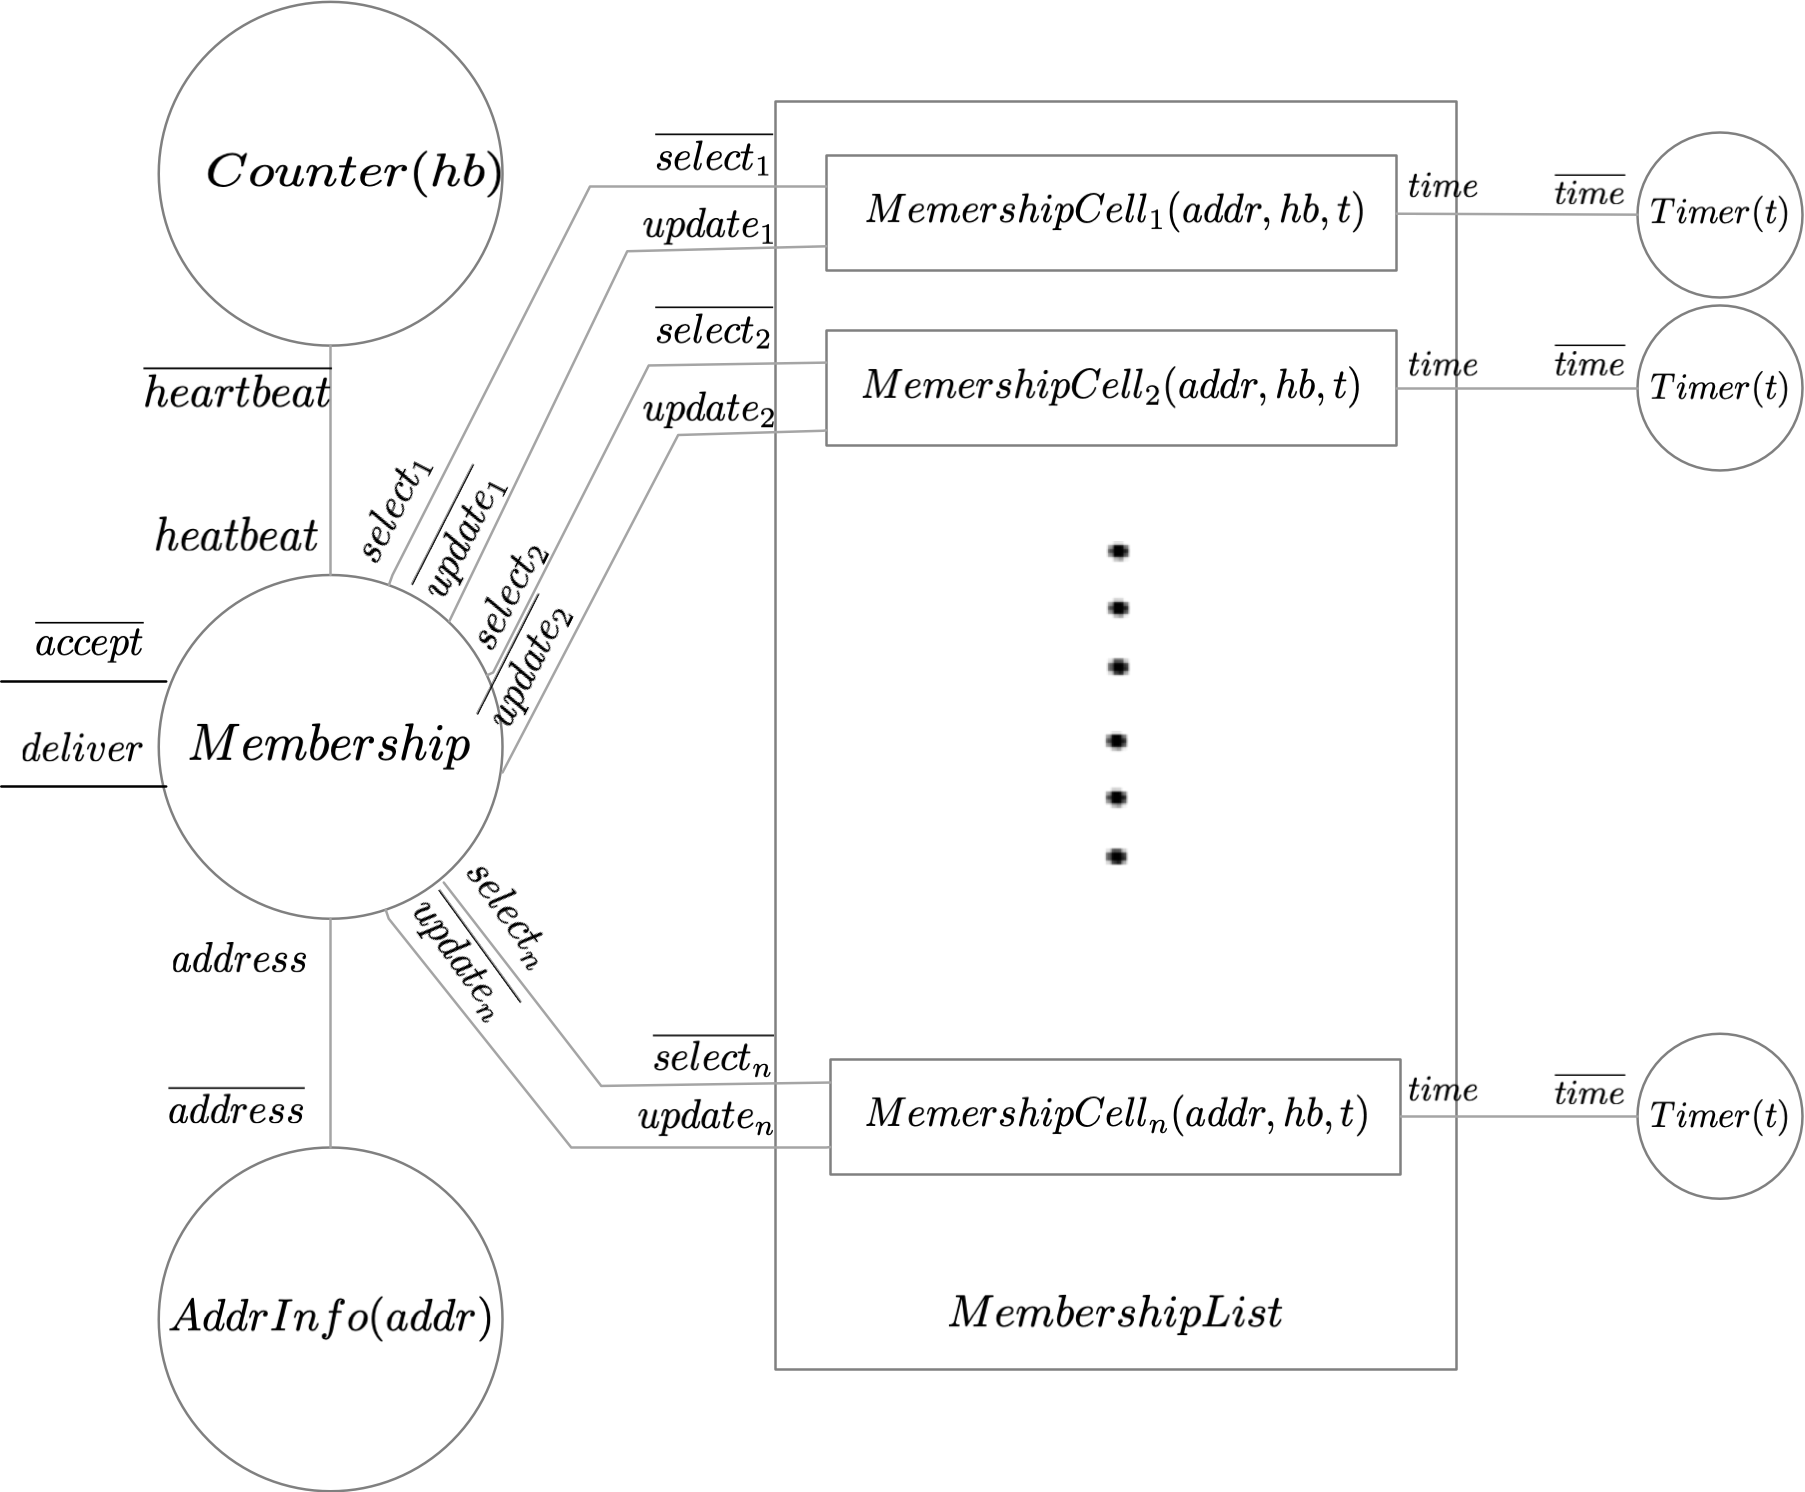
\includegraphics[width=11cm]{../figures/membership.png}
    \caption{Membership示意图}
    \label{fig:membership_system}
\end{figure}
可以看到,我们使用$n$个$MembershipCell$来存储Membership List中的每一项,
$Membership$可以通过$select_i$通道获取$MembershipCell_i$中的数据,
也可以通过$update_i$通道更新$MembershipCell_i$中的数据,
每一个$MembershipCell$连接一个Timer,用来获取本地时间,设置LocalTime字段,
实际上,对于一个节点它可能只有一个Timer,这里的连接也是指逻辑连接。
$MembershipCell$的定义如下:
\begin{equation}
   \begin{split}
      &MembershipCell_i(addr,hb,t)\stackrel{def}{=}\\
   &\quad\overline{select_i}(\{Address:addr,HeartBeat:hb\}).MembershipCell_i(addr,hb,t)\\
   &\quad+update_i(\{Address:addr',HeartBeat:hb'\}).time(t').MembershipCell_i(addr',hb',t')
   \end{split}
\end{equation}
$n$个并发的$MembershipCell$组成的$MembershipList$定义如下,
在初始状态时,每一个$MembershipCell$中的数据为空($\epsilon$):
\begin{equation}
   MembershipList\stackrel{def}{=}(MembershipCell_1(\epsilon)\mid \dots MembershipCell_n(\epsilon))
\end{equation}

此外,我们定义了一个$Counter$维护和更新节点的心跳计数,
在每一次Gossip周期$hb=hb+1$,
$Membership$可以通过$heartbeat$通道获取心跳。
\begin{equation}
   Counter(hb)\stackrel{def}{=}\overline{heartbeat}(\mathsf{s}(hb)).Counter(\mathsf{s}(hb))
\end{equation}

对于节点本地地址的维护,我们定义了一个$AddrInfo$来储存本地地址,
$Membership$可以通过$address$通道获取本地地址。
\begin{equation}
   AddrInfo(addr)\stackrel{def}{=}\overline{address}(addr)
\end{equation}

定义完以上的辅助工具后,我们可以定义$Membership$的逻辑了!
\begin{equation}
   \begin{split}
    &Membership\stackrel{def}{=}address(addr).heartbeat(hb).select_1(x_1)\dots select_n(x_n).\\
    &\quad\overline{accept}(\{Address:addr,HeartBeat:hb\},x_1,\dots,x_n).Membership\\
    &\quad+deliver(x_1,x_2,\dots,x_n).Processing(x_1,x_2,\dots,x_n)\\
    &Processing(x_1,x_2,\dots,x_n)\stackrel{def}{=}(Check(x_1)\mid  \dots \mid Check(x_n) \mid Membership)\\
    &Check(x)\stackrel{def}{=}address(addr).((addr=x[Address])0|\urcorner(addr=x[Address])FindAndUpdate_1(x))\\
    &FindAndUpdate_i(x)\stackrel{def}{=}select_i(x_i).((x_i = \epsilon) (\overline{update_i}(x).0)\\
    &\quad\mid \urcorner(x_i = \epsilon)((x_i[Address]=x[Address])((x_i[HeartBeat]<x[HeartBeat])(\overline{update_i}(x).0)\\
    &\quad\mid \urcorner (x_i[HeartBeat]<x[HeartBeat])0)\\
    &\quad\mid \urcorner (x_i[Address]=x[Address])FindAndUpdate_{i+1}(x))),i\leq n\\
    &FindAndUpdate_i(x)\stackrel{def}{=}0,i>n
    \end{split}
\end{equation}
其中$\mathsf{s}(x)$表示$\mathsf{s}(x)=x+1$,$\mathsf{s}(x)$的实现可以通过FU Y在The Value-Passing Calculus中定义的Numeric System实现\cite{Fu_VPC}。

$Membership$可以获取$MembershipList$中所有Cell中储存的信息,
添加本地地址和心跳后,将这一组信息经$accept$通道发出,
根据$Node$的定义,我们知道$Node$从$accept$通道接受这些信息后会随机的发送给$k$个其他节点。
另外,$Membership$从$deliver$通道接收了其他节点发送的Membership List后,
将迁移到状态$Processing(x_1,x_2,\dots,x_n)$。
$Processing(x_1,x_2,\dots,x_n)$可以并发的运行$Check(x_i)$,
在$Check(x_i)$状态下,
若$x_i$的地址为当前节点的地址,不做处理,
若不为当前节点的地址,
则从第一个$MembershipCell$开始对比$x_i$的地址与$MembershipCell$的地址,
若地址相同且$x_i$中的心跳计数大于$MembershipCell$中的心跳计数,
更新$MembershipCell$的数据;
若所有有值的$MembershipCell$均无$x_i$的地址,用$x_i$直接更新第一个空的Cell。

\section{基于Gossip-Style Membership协议的通信系统的仿真模拟}
在本节我们会根据本章的模型来实现一个基于Gossip-Style Membership协议的P2P系统,
由于资源限制,不能实际部署在多个主机构成的集群,我们将使用多进程来模拟多个主机,
实际上进程理论本就是用来刻画进程的并发,多个主机上的程序的本质也是进程。

\subsection{Go语言与CSP}
我们将使用Go语言实现这个基于Gossip-Style Membership协议的通信系统,
Go语言实现了两种并发模型,一种是C++,Java使用的多线程,一种是CSP\cite{Hoare_CSP}并发模型。
如我们在第~\ref{ch:intro}章中提到的,
CSP也是一种经典的进程演算,它与CCS的区别在于等价的类型和建模并发系统采用的方法,有关CCS和CSP对比的研究也有很多\cite{DIFF_CCS_CSP,CCS_CSP1,CCS_CSP2,CCS_CSP3}。
Go语言使用了CSP理论中的Process/Channel,对应到语言特性中的 goroutine/channel\cite{Golang}。
Goroutine是一种轻量级线程,channel用于协程间的通信。
我们使用Go语言的并发特性可以更加直观的展示出对前述模型的代码实现。

% CSP也是一种进程演算,
% 与CCS存在相似和差异[cite],
% 本实现主要利用了Go语言的通道特性,
% 通道的概念是CSP的组成部分,
% 在CCS中对应端口的概念,其本质是相似的。
% 使用Go语言的通道可以更加直观的展示出对上述模型的代码实现。

\subsection{代码实现与仿真效果}

 由于代码的解释比较枯燥,本小节只展示关键部分的代码实现,
 完整的代码实现及下载、运行方式可以参考附录~\ref{app:code}。
 在编写代码的过程中,考虑到代码的可读性和字符的限制,
 我们对前述模型通道和进程状态的名称有所修改,
 但本质没有变化。

 在Go语言中,我们可以用channel特性来实现$\mathbb{RVPC}_{\mathsf{Th}}$中的通道。
 如在实现Gossip-Style Membership的节点结构时,
 Node结构体中,chan类型的字段分别
 代表了图~\ref{fig:membership_node}中的相应名字的通道。
 其中,我们在~\ref{ch:gossip_impl}小节中提到
 $trans_{i,j}$通道用于节点$i$向节点$j$传输信息,
 这一通道实质上表达的是信息传输的逻辑路径,
 我们在实现时考虑信息传输的代码层面的物理路径,
 只需要每一个节点设置一个
 $trans$通道用于接收集群中其他节点的信息即可,
 向其他节点发送信息时,我们可以通过Others字段向
 Others[i].trans通道发送消息。
 对于Node节点的状态迁移,我们可以使用bool类型的字段isbad表示节点状态是否为BadNode。
 \begin{codeblock}[language=GO]
   type Node struct {
      isbad bool
      trans chan []Message
      time chan Nil
      timeout chan Nil
      accept chan []Message
      deliver chan []Message
      Others []*Node
   }
\end{codeblock}

我们可以使用基于select的多路复用实现非确定性选择,
如我们在~\ref{eq:network_system}中实现的系统中的$Node_i$:
这里$Node_i$可以做非确定的选择:
接收到timeout信号后从accept通道获取本地的Membership List
随机选择$k$个其他节点发送;或从其他节点接收到Membership List消息,
通过deliver通道向本地的Membership进程传递该消息。

\begin{codeblock}[language=GO]
   select {
      //timeout.accept(x).bigoplus p tau.GossipingNode
      case <- node.timeout:
         messages := <- node.accept
         //随机生成k个其他节点的排列targets
         node.Gossiping(messages, targets)
      // sum trans(x).deliver(x).FragileNode
      case message := <- node.trans:
         node.deliver <- message
	}
\end{codeblock}
select的语法与switch比较相似,
每一个case代表一个通信操作,
select会等待case中有能够执行的case时执行该case:
当条件满足时,select才会通信并执行case后的语句块,
其他通信不执行。

在Go语言中,每一个并发执行的单元称为一个goroutine,
我们同样使用goroutine来实现$\mathbb{RVPC}_{\mathsf{Th}}$
中的并发。
如对$GossipSystem_\mathsf{N}\stackrel{def}{=}(FragileNode_1\mid FragileNode_2\mid \dots \mid FragileNode_n)$,
的实现:
\begin{codeblock}[language=GO]
   for i:=0;i<NODE_NUM;i++ {
        go nodes[i].Fragile()
    }
\end{codeblock}
实际上在我们的系统中,对一个节点本地的Timer,Membership和接入通信网络的Node
同样应该是并发的。

本节仿真实现的基于Gossip-Style Membership协议的P2P系统参数如表~\ref{tab:param}。
\begin{table}[!hpt]
   \caption{基于Gossip-Style Membership协议的P2P系统参数表}
   \label{tab:param}
   \centering
   \begin{tabular}{@{}ccc@{}} \toprule
   %   \multicolumn{2}{c}{Item} \\ \cmidrule(r){1-2}
     参数名称 & 参数值 & 参数含义 \\ \midrule
     $n$ & 5 & 系统节点数量\\
     $k$ & 2 & 每Gossip周期发送的节点数\\
     $T_{Gossip}$ & 1s & Gossip周期\\
     $T_{repair}$ & 4s & 失效节点恢复时间\\
     $T_{fail}$ & 4s & 节点有效期超时时间\\
     $p_{fail}$ & 0.1 & 节点失效概率\\ \bottomrule
   \end{tabular}
 \end{table}

 我们使用上述参数运行我们实现的系统,
 我们使用html为我们的系统做了一个前端界面,
 我们可以在这个界面观察每个节点Membership List的更新过程。

 \begin{figure}[!htp]
   \begin{minipage}{0.9\textwidth}
     \centering
     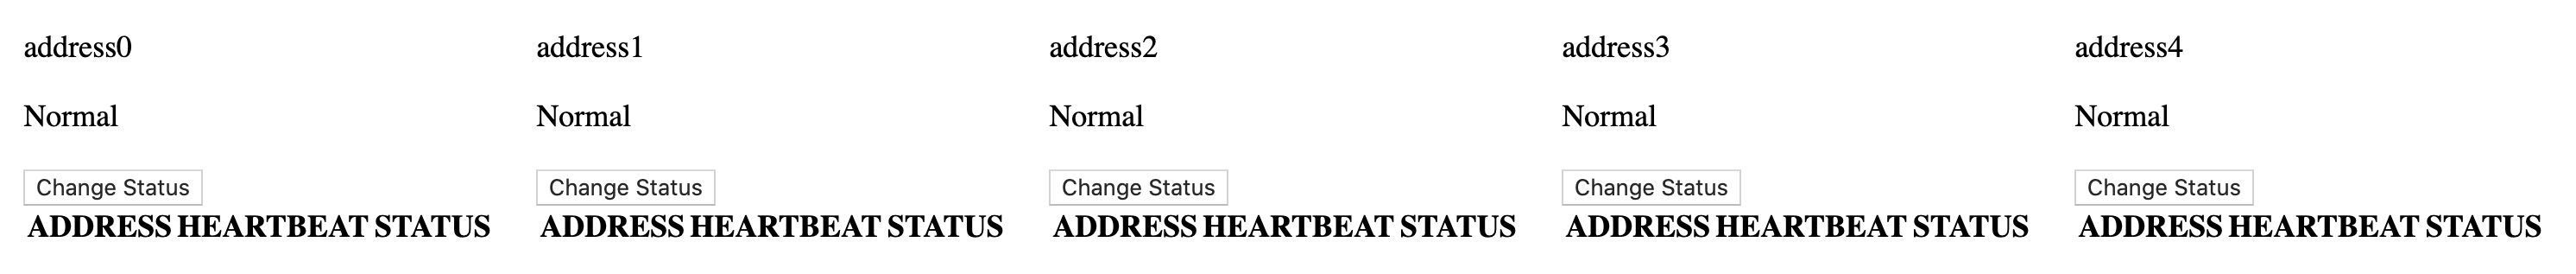
\includegraphics[width=15cm]{../figures/demo/4.png}
     \\
     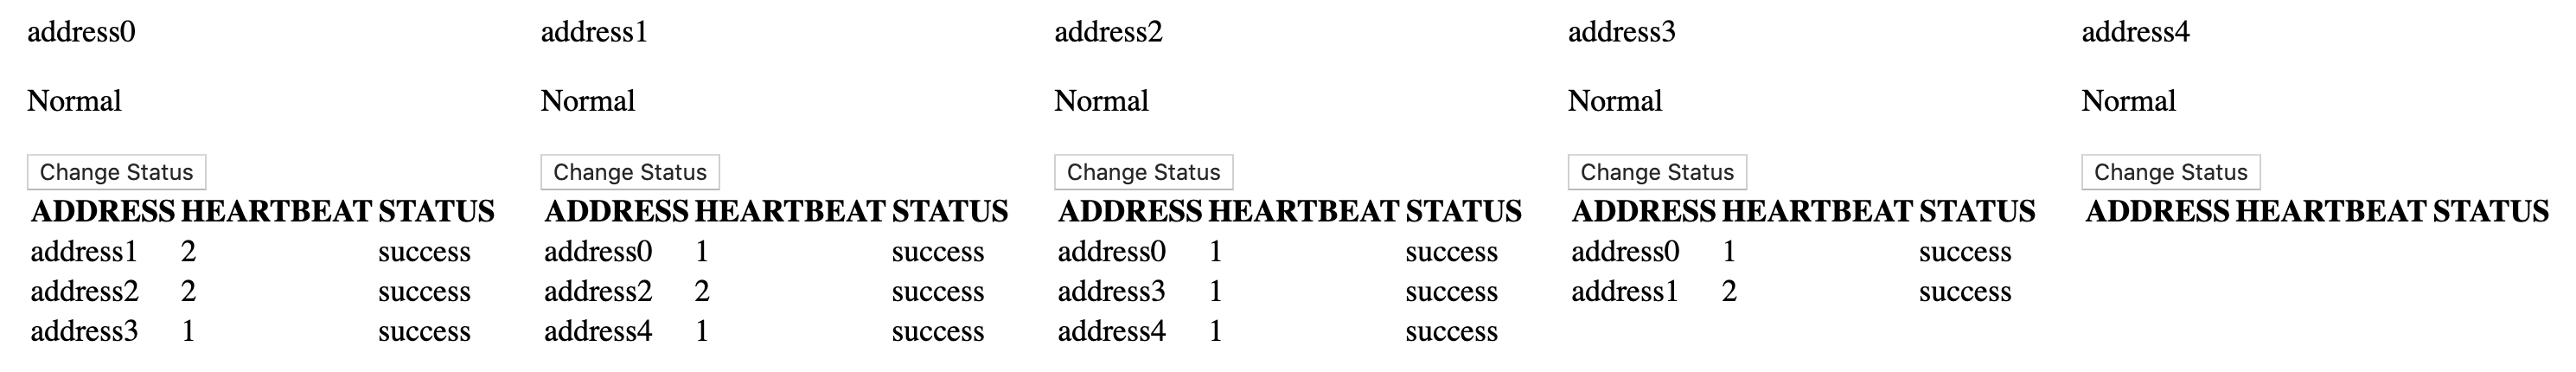
\includegraphics[width=15cm]{../figures/demo/5.png}
     \\
     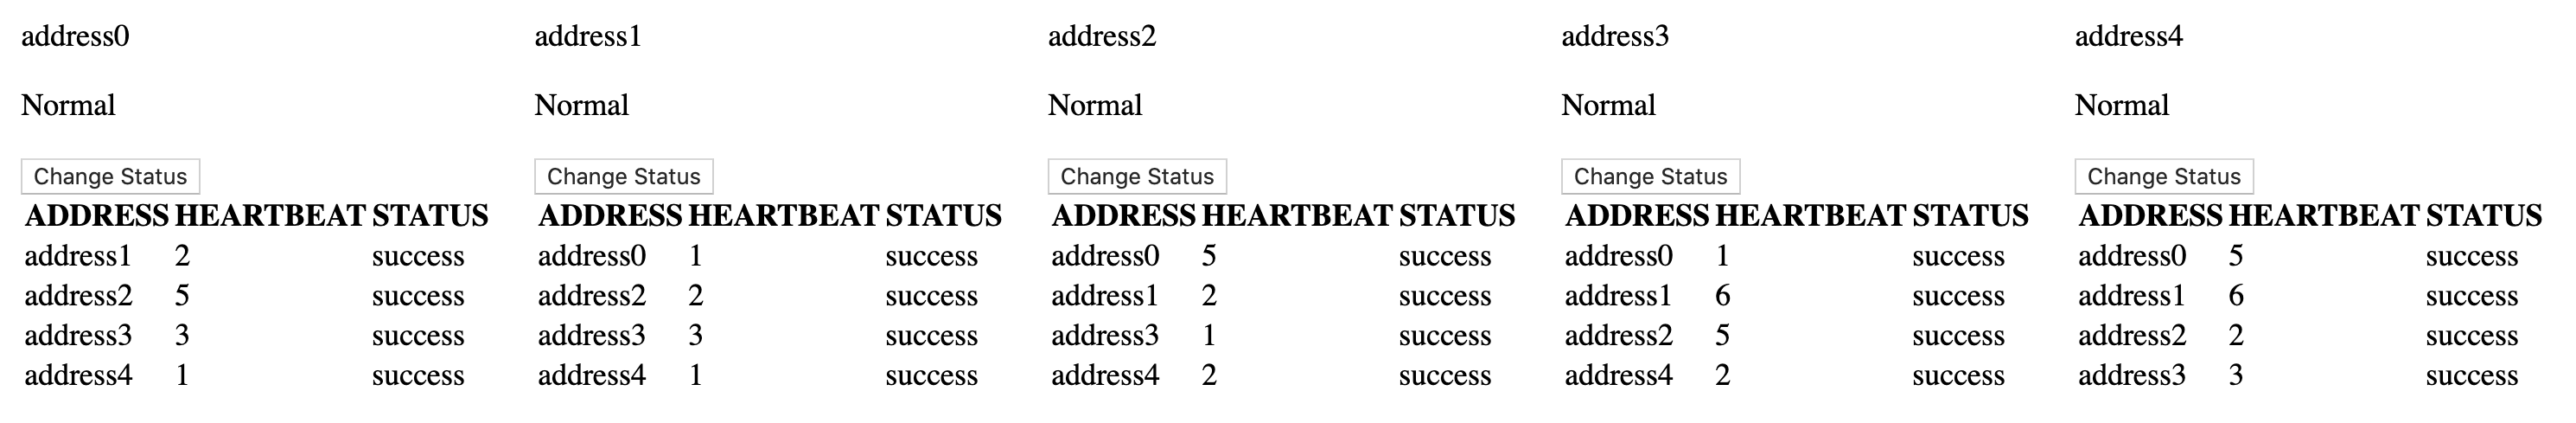
\includegraphics[width=15cm]{../figures/demo/6.png}
   \end{minipage}
   \caption{基于Gossip-Style Membership协议的5节点P2P系统的Membership List扩展过程}
   \label{fig:demo_1}    
\end{figure}
 图~\ref{fig:demo_1}展示了每个节点的Membership List的扩展过程,
 其中第一行为节点的地址,我们使用字符串表示,也可以根据需要修改成其他的形式,
 第二行为对应节点的状态,Bad表示节点失效,对应$BadNode$状态,
 Normal表示节点正常,对应$FragileNode$和$Node$状态,
 第三行的按钮可以改变节点的状态,
 接下来的是对应节点的Membership List,可以看到我们展示了Address,Heartbeat, Status字段,
 其中Status字段是由LocalTime计算而得,
 当当前时间与Membership List项的LocalTime字段相差超过$T_{fail}$时,我们认为这一项对应的节点处于失效状态。
 在~\ref{fig:demo_1}的第一个图中,我们可以看到初始状态所有节点的Membership List为空,
 第二张图中Membership List进行了扩张,第三张图中全部节点的Membership List包含了所有其他节点。

我们同样可以展示系统的失效检测。在图~\ref{fig:demo_2}中,
第一张图是正常状态,
我们在第二张图中手动改变了地址为address1节点状态,使该节点失效,
可以看到第三张图中address0,address3检测到了address1的失效,
第四张图所有节点都检测到了address1的失效。
 \begin{figure}[!htp]
   \begin{minipage}{0.9\textwidth}
     \centering
     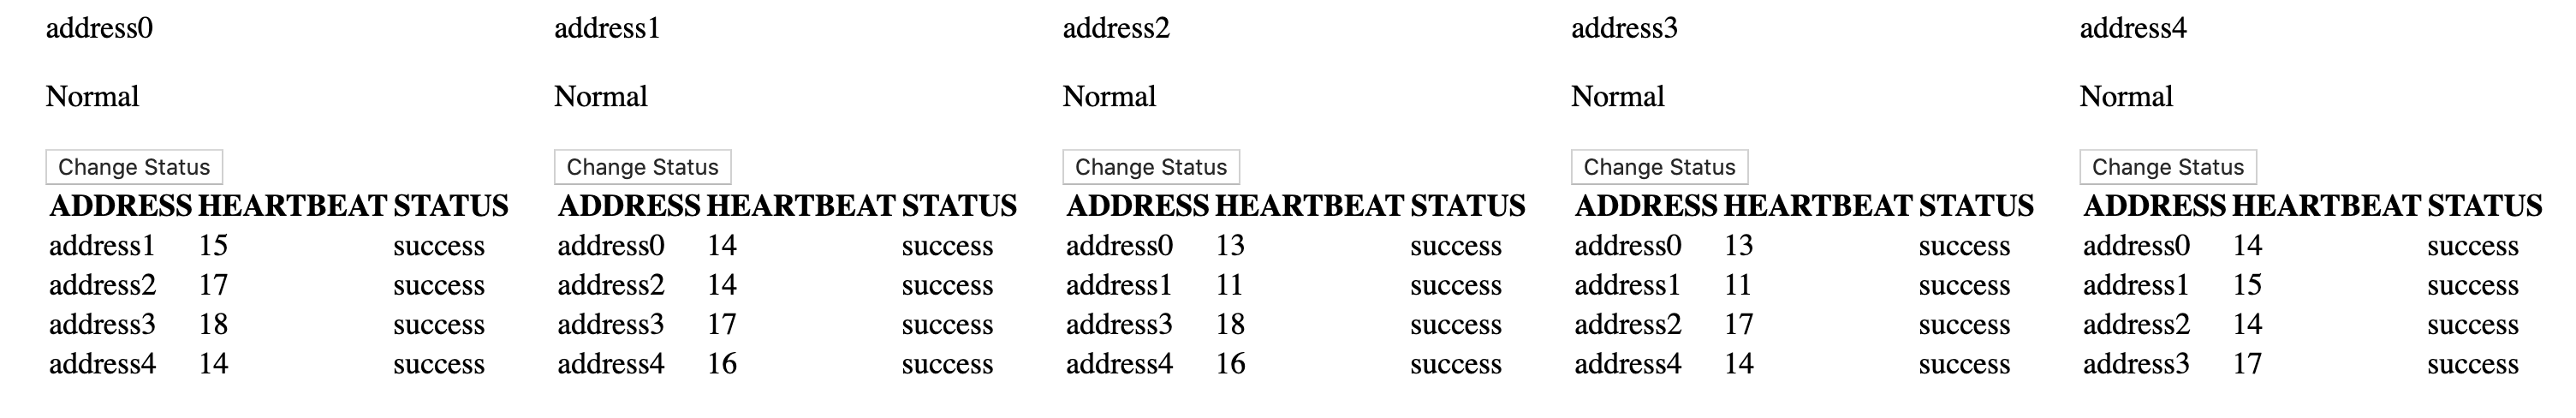
\includegraphics[width=15cm]{../figures/demo/0.png}
     \\
     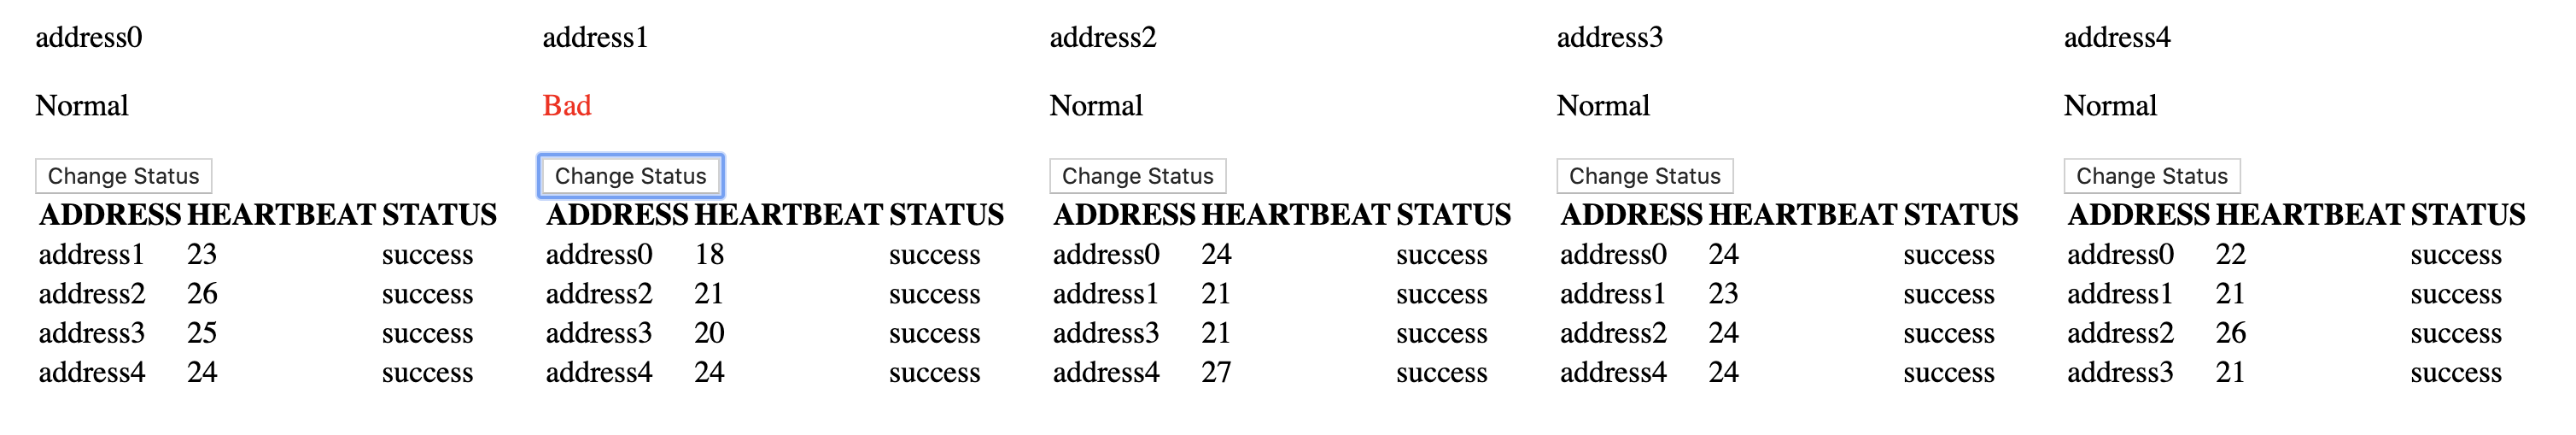
\includegraphics[width=15cm]{../figures/demo/1.png}
     \\
     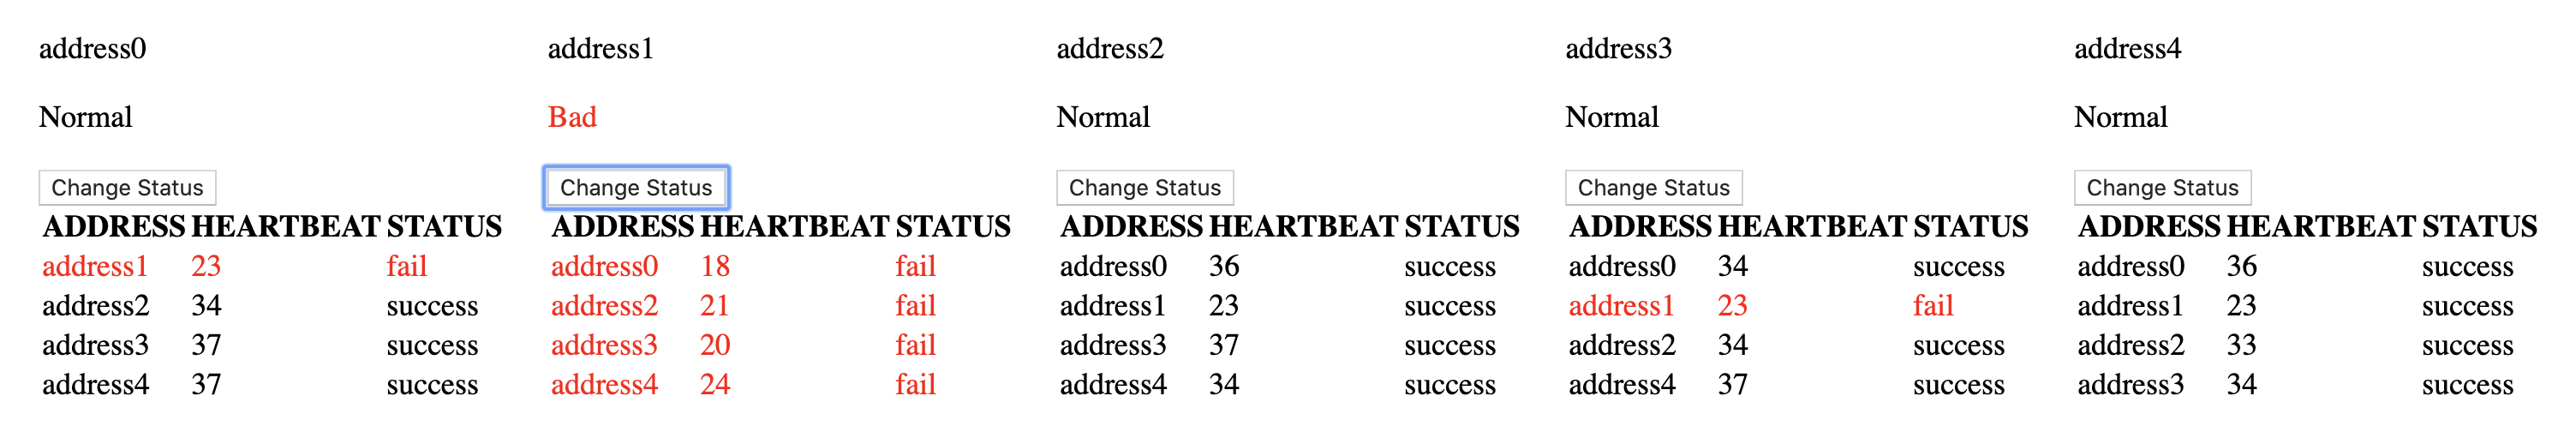
\includegraphics[width=15cm]{../figures/demo/2.png}
     \\
     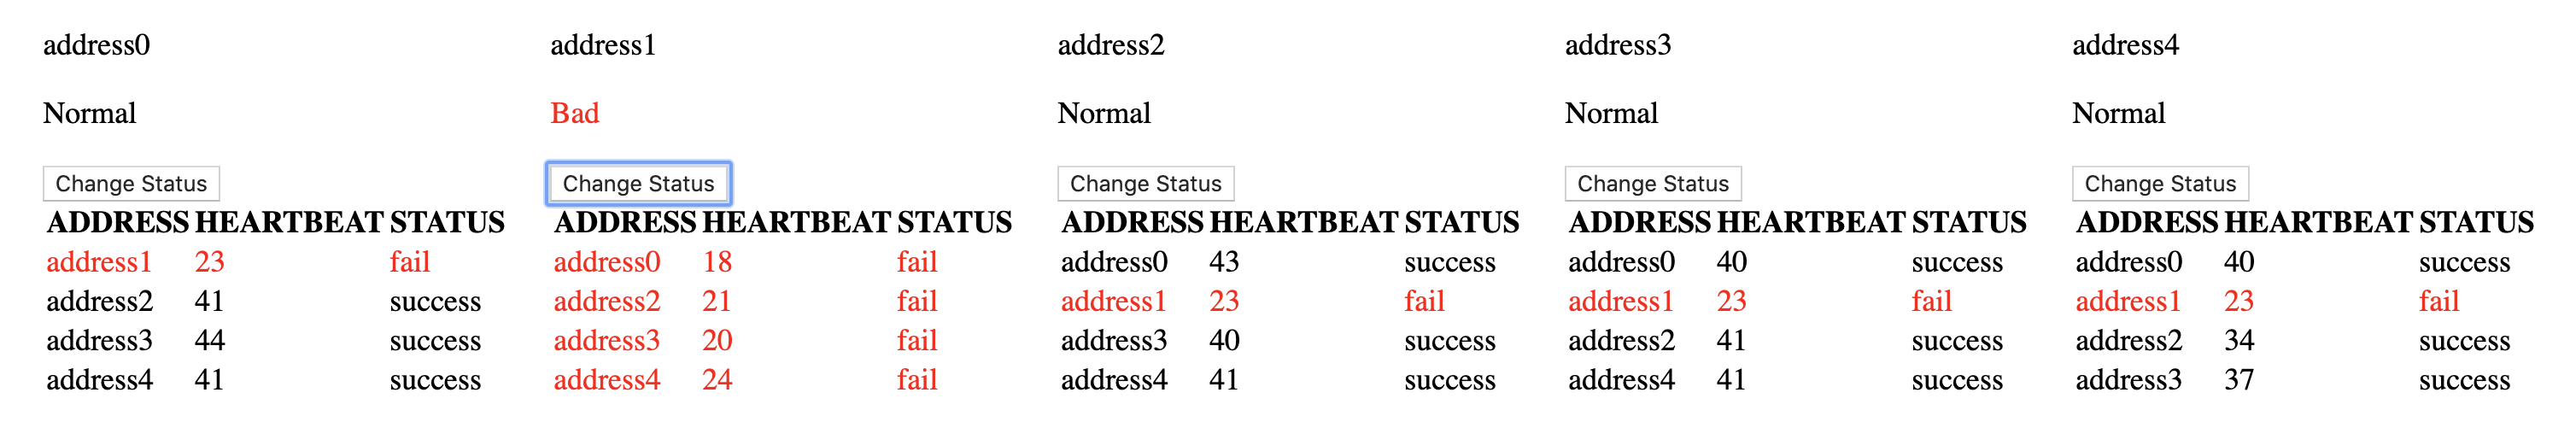
\includegraphics[width=15cm]{../figures/demo/3.png}
   \end{minipage}
   \caption{基于Gossip-Style Membership协议的5节点P2P系统的错误检测}
   \label{fig:demo_2}   
\end{figure}

我们也可以通过设置$p_{fail}$使系统中的节点以一定概率自动失效和恢复,
动态效果可以通过附录~\ref{app:code}中的方式获得。

 \section{本章小结}
 本章我们以一种基于云计算失效检测协议Gossip-Style Membership协议的通信系统的
 $\mathbb{RVPC}_{\mathsf{Th}}$实现作为
 本文中提出的随机传值进程模型的应用案例,
 提供了使用$\mathbb{RVPC}_{\mathsf{Th}}$建模及实现通信协议以至其他现实问题的思路。

 我们首先介绍了Gossip协议和Membership协议,
并使用$\mathbb{RVPC}_{\mathsf{Th}}$实现了基于Gossip协议的P2P系统,
使用$\mathbb{RVPC}_{\mathsf{Th}}$的符号互模拟证明了Gossip协议与多播规约的观察等价性。
在基于Gossip协议的P2P系统的基础上,我们修改实现使其成为基于
Gossip-Sytle Membership协议的P2P系统,并给出了GO语言的代码实现和仿真模拟。
仿真结果证明了我们的随机传值进程模型在对并发通信过程的建模和分析中有一定的可行性。
